\documentclass[a4paper,10pt]{article}
\usepackage{hyperref}
\usepackage{setspace}
\usepackage{graphicx}
\usepackage{color}
\usepackage{xcolor}
\usepackage{relsize}
\usepackage{listings}
\usepackage[round]{natbib}
\usepackage{minted}
\usepackage{float}
\hypersetup{colorlinks = true, linkcolor = blue}
\lstset{language=Python}
\usepackage[margin=0.5in]{geometry}

\usepackage{listings}
\usepackage{makeidx}
\usepackage{titlesec}
\setcounter{tocdepth}{5}
\usepackage[T1]{fontenc}
\usepackage[utf8]{inputenc}
\usepackage{authblk}
\makeindex{}
%\VignetteEngine{knitr}
%\VignetteIndexEntry{A Markdown Vignette with knitr}
\definecolor{bg}{rgb}{0.95,0.95,0.95}


\title{\textbf{A bioinformatics workflow for detecting signatures of selection in genomic data}}
\date{September 9, 2013}

\author[1,2]{Murray Cadzow}
\author[1,2]{James Boocock}
\author[1,2]{Hoang Tan Nguyen}
\author[2,3]{Phillip Wilcox}
\author[1]{Tony R Merriman}
\author[1]{Michael A Black}
\affil[1]{Department of Biochemistry, University of Otago}
\affil[2]{Department of Mathematics and Statistics, University of Otago}
\affil[3]{Scion Research, Rotorua, New Zealand}
\renewcommand\Authands{ and }
\begin{document}

\maketitle{}
\doublespacing
\tableofcontents
\section{Introduction}
The SelectionPipeline Program utilizes next-generation sequencing \(NGS\) data to generate selective signatures. The tools used to detect selection are dependent on the selection signature being investigated \citep{Sabeti:2006ha}. The pipeline generates various output files within and between populations. The starting point for the analysis is a variant call format \(VCF\) file of the genotype data and populations of interest \citep{Danecek:2011gz}. Both $F_{st}$ and Tajima's D can be calculated from standard genotype data \citep{Weir:1984vn} \citep{Tajima:1989un}. To compute iHS, rsb and Fay and Wu's requires haplotypes, and thus the genotype data must be phased prior to calculation of these statistics \citep{Voight:2006go} \citep{Gautier:2012et} \citep{fayandwush}. For phasing shapeit2 is used and for imputation impute2 is used \citep{impute22009} \citep{Delaneau:2013hi}. Furthermore these statistics need ancestral allele information. The pipeline phases if the VCF files do not contain the phasing information and then performs ancestral allele annotation. Once complete, the rehh package provides a simple interface for implementing EHH-based analyses \citep{Gautier:2012et}, we extended rehh to include parameters that match those used in \emph{Voight et als.} seminal paper \citep{Voight:2006go}, rehh calculates iHH, iHS, iES and Rsb. To calculate Fay and Wu's H we used a c program called variscan \citep{variscan2005}. The pipeline implemented in python, takes a VCF file to a set of output files containing selection signatures.
\section{Getting Started}
\subsection{Prerequisites}
The selection pipeline was developed on a 64-bit ubuntu 13.04 system but should work on any 64-bit linux deriviant assuming some basic libraries and tools are installed on your system. 20gb of ram should be sufficient \(required for imputation\).
\begin{itemize}
\item python2 > 2.7 
\item bourne-again Shell (Bash)
\item perl5
\end{itemize}
\subsection{Installation}
To install the package standalone, requiring manual configuration of the config file run the following command.\\

\begin{minted}[bgcolor=bg,frame=lines]{bash}
./install.sh --standalone
\end{minted}

The rest of this section will be dedicated to the automatic installation. To perform an automatic installation of the selection pipeline run the command.\\
\begin{minted}[bgcolor=bg,frame=lines]{bash}
./install.sh
\end{minted}

Installation creates a default configuration file located in the base directory of the pipeline. Installation adds a program called selection\_pipeline to the system path. To test the program is installed correctly run the following command at a terminal prompt.

\begin{minted}[bgcolor=bg,frame=lines]{bash}
selection_pipeline -h
\end{minted}

\subsection{Genetic Maps and Impute Haplotypes}
To use the phasing and imputation features of the pipeline requires both genetic map files and haplotype files. For humans these files that conform to the format required for shapeit and impute2 can be found \href{http://mathgen.stats.ox.ac.uk/impute/impute_v2.html#reference}{here}. For impute2 one reference is available \href{http://mathgen.stats.ox.ac.uk/impute/ALL_1000G_phase1integrated_v3_impute_macGT1.tgz}{here}, download and extract the archive to referencefiles/impute\_ref and uncompress the contents. For shapeit2 a genetic map can be found \href{http://www.shapeit.fr/files/genetic_map_b37.tar.gz}{here}, download and extract the archive to referencefiles/shapeit\_ref.\\

To use other reference files with the selection pipeline requires setting a few options in the config file. The question mark character "?" in the config is substituted by the chromosome number, this is used for reference files that are split on chromosomes.\\
\begin{minted}[bgcolor=bg,frame=lines]{bash}
...
genetic_map_prefix=genetic_map_chr?_combined_b37.txt
...
impute_map_prefix=genetic_map_chr?_combined_b37.txt
impute_reference_prefix=ALL_1000G_phase1integrated_v3_chr?_impute
...
\end{minted}

If you decide to store you reference files in another location, further options will require alterations.\\ 
\begin{minted}[bgcolor=bg,frame=lines]{bash}
...
genetic_map_dir= \${HOME}/MerrimanSelectionPipeline/referencefiles/shapeit_ref
...
impute_map_dir= \${HOME}/MerrimanSelectionPipeline/referencefiles/impute_ref
impute_reference_dir= \${HOME}/MerrimanSelectionPipeline/referencefiles/impute_ref
...
\end{minted}

\subsection{Ancestral Fasta Files}
The generation of results for iHS requires assigning the ancestral allele. The selection pipeline uses the ancestral alleles from the 6-way EPO (Enredo-Pecan-Ortheus) alignment pipeline. The files can be downloaded from \href{ftp://ftp.1000genomes.ebi.ac.uk/vol1/ftp/phase1/analysis_results/supporting/ancestral_alignments/human_ancestor_GRCh37_e59.tar.bz2}{here}. Make sure to extract contents of the archive after download. The default directory to store the ancestral reference files is referencefiles/ancestral\_ref/.

If you downloaded your reference to a different location you can set the following setting in your config file.\\
\begin{minted}[bgcolor=bg,frame=lines]{bash}
...
ancestral_fasta_dir = # directory you downloaded alignment to #
...
\end{minted}

\section{Tutorial}
\subsection{Selection Signatures at the Lactase Locus}
\subsubsection{Getting the Data}
The lactase gene is located on Chromosome 2 between 136,545,410-136,594,750 positions. For the example we will use a 10 megabase region containing the Lactase gene and the CEU and YRI populations from the 1000 genomes. In order to demonstrate how to use the pipeline we will use the chromosome 2 region 130,000,000-140,000,000. To download the example dataset enter the command below. The lactase gene is an example of strong selection in the last 5,000-10,000 years in human populations specifically European-derived populations (cite).  \\

\begin{minted}[bgcolor=bg]{bash}
wget http://tutorial_file_location.com 
\end{minted}

Extract the example data into a new folder.

\subsection{Setting up Pipeline Run}
\subsection{Population Files}
Population files are required for any cross population comparisions. The commands below will initiate the data generation step. Population files are line seperated files the first line contains the population name every successive line contains and individual ID from that population.\\
\subsection{Run The Tutorial}
The default configuration file is located in the base directory of the selection pipeline. To run the pipeline run the command below in the folder you extracted the example data and change the --config-file parameter to match the location you have installed the pipeline.\\
\begin{minted}[bgcolor=bg,frame=lines]{bash}
multipop\_selection_pipeline -p CEU_ids.txt -p YRI_ids.txt 
-i CEU_YRI_lactase.vcf --config-file defaults.cfg
--fst-window-size 1000 --fst-window-step 1000
\end{minted}
The generated folders and current folder have all the data required to perform further selection analysis. Within each population folder 4 output files are generated these contain Tajima's D, iHH, an updated VCF and Fay and Wu's H statistic these files are located in the results folder inside each population subfolder. Fst is calculated between each population and results are located in the fst folder. Fst results are calculated using the Weir and Cockerham estimator.
\subsection{Data Visualisation}
The purpose of the pipeline is to generate standard signatures of selection from a VCF formatted input file. In order to express the usefulness of the pipeline it is pertinent to illustrate the effectiveness of the pipeline. The next section describes some basic plotting of these data using the R programming language. All following commands are run in a R session with the working directory in the base directory you are running the tutorial in. In each case the blue lines outline the lactase gene.
\subsubsection{Fst}


\begin{minted}[bgcolor=bg,frame=lines]{r}
CEUYRIfst=read.table("fst/2CEUYRI.fst", header=TRUE)
# Plot FST 1 megabase each side of the lactase gene
# Plot the weighted fst value for each region
plot(CEUYRIfst[,5]~CEUYRIfst[,2], pch=16, cex=.4, type="p",xlab='',ylab='FST') 
rect(136545410,0,136594750,1,border="Blue") 
\end{minted}

\begin{figure}
\centering
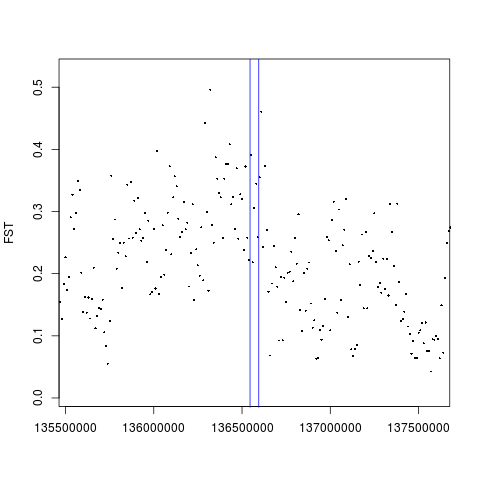
\includegraphics{pictures/CEUYRI2.png}
\caption{CEU YRI Fst Values}
\label{fig:a}
\end{figure}
Figure~\ref{fig:a} shows clustering of high FST values close to the lactase gene plotting one megabase downstream and upstream either side of the gene. 
\subsubsection{Fay and Wu's H}
To plot the Fay and Wu's H values for the CEU population.\\
\begin{minted}[bgcolor=bg,frame=lines]{r}
CEUFay=read.table('CEU/results/CEU2.faw',comment.char="#")
#Plot Fay and Wu's H
plot(CEUFay[,15] ~ CEUFay[,1],xlim=c(136545410-1e6,136594750+1e6),pch='.',cex=2,
xlab='',ylab="H Statistic")
rect(136545410,-100,136594750,100,border="Blue") 
\end{minted}
\begin{figure}
\centering
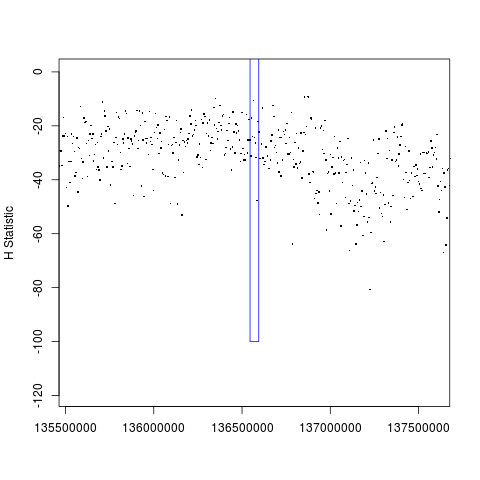
\includegraphics{pictures/CEUFay.png}
\caption{CEU Fay and Wu's H}
\label{fig:fay}
\end{figure}
Figure~\ref{fig:fay} show the Fey and Wu's H statistic one megabase downstream and upstream of the lactase gene

\subsubsection{iHS}
To plot the iHS values around the lactase gene for the CEU population.\\
\begin{minted}[bgcolor=bg,frame=lines]{r}
CEUihs = read.table('CEU/results/CEUchr2.ihs')
#plot IHS pvalues
plot(CEUihs[,4] ~ CEUihs[,2],xlim=c(136545410-1e6,136594750+1e6),pch='.',cex=2)
rect(136545410,-10,136594750,10,border="Blue") 
\end{minted}

\begin{figure}
\centering
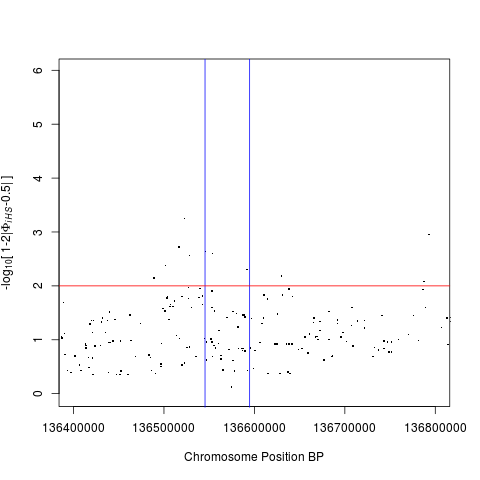
\includegraphics{pictures/CEUihs.png}
\caption{CEU IHS}
\label{fig:b}
\end{figure}

Figure ~\ref{fig:b} shows iHS pvalues around the lactase gene one megabase upstream and downstream.

\subsubsection{Tajima's D}
\begin{minted}[bgcolor=bg,frame=lines]{r}
tajimaD=read.table(file="CEU/results/CEU2.taj_d", header=TRUE)
plot(tajimaD[,4] ~ tajimaD[,2],xlim=c(136545410-1e6,136594750+1e6),pch='.',cex=2)
rect(136545410,-10,136594750,10,border="Blue") 
\end{minted}

\begin{figure}
\centering
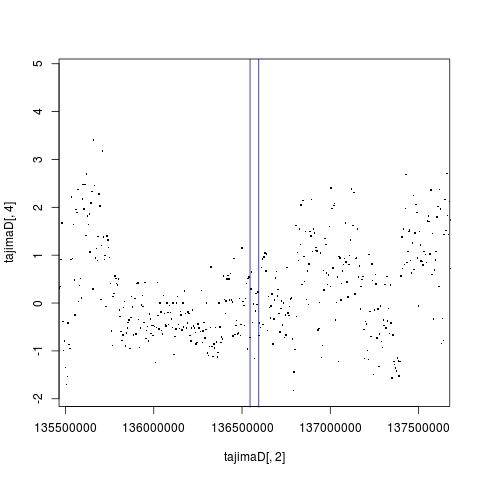
\includegraphics{pictures/CEUtajimas.png}
\caption{CEU IHS}
\label{fig:taj}
\end{figure}

Figure~\ref{fig:taj} show the Tajima's D statistic one megabase downstream and upstream of the lactase gene


\subsubsection{Rsb}
\begin{minted}[bgcolor=bg,frame=lines]{R}
\end{minted}
\section{Output Files}
The output files are preserved in the same state as the original output from the program used to generate the data.
\subsection{multi\_population}
\subsubsection{Fst}
Located in the fst folder. Tab-delimited data file containing 1 header line followed data on each subsequent line\\
\begin{minted}[bgcolor=bg,frame=lines]{rst}
CHROM   BIN_START       BIN_END N_VARIANTS      WEIGHTED_FST    MEAN_FST  
2       130000001       130010000       94      0.133102        0.0680276 
\end{minted}
\subsection{selection\_pipeline}
All the outputs for each population are contained in the results folder. If you ran the tool using \emph{multi\_population} the outputs are located in <pop name>/results. 
\subsubsection{Fay and Wu's H}
Space-delimited data file containing header line that start with a hash character (\#). Contains lots of columns if you are only interested in Fay and Wu's H, column 1 provides the position and column 15 provides the H statistic. \\
\begin{minted}[bgcolor=bg,frame=lines]{rst}
# RefStart   Refend ... FayWu\_H
130000040 130005039 ... -22.2438460
\end{minted}
\subsubsection{iHS}
Space-delimited data file containing one header line followed by data on each subsequent line.\\
\begin{minted}[bgcolor=bg,frame=lines]{rst}
"CHR" "POSITION" "iHS" "Pvalue"
"rs4662641" 2 130000272 0.0644902912148128 0.0229261107107533
\end{minted}
\subsubsection{iHH}
Space-delimited data file containing one header line followed by data on each subsequent line.\\
\begin{minted}[bgcolor=bg,frame=lines]{rst}
"CHR" "POSITION" "FREQ_a" "IHHa" "IHHd" "IES"
"rs1251176" 2 130000040 0.9823 11558.89 83915.49 11571.13
\end{minted}
\subsubsection{Tajima's D}
Space-delimited data file containing one header line followed by data on each subsequent line.\\
\begin{minted}[bgcolor=bg,frame=lines]{rst}
CHROM   BIN\_START       N\_SNPS  TajimaD
2       130000000       22      0.775224
\end{minted}

\section{Command line Arguments}
The selection pipeline contains three programs: \emph selection\_pipeline,\emph aa\_annotate, and\emph multipopulation. The selection pipeline does all the intra-population statistics calculations. The multipopulation program calculates all the inter-population statistics and calls the selection pipeline. The aa\_annotate program annotates a haplotype file or a phased vcf file with the ancestral allele from the 6-way EPO alignment, for other species or alternative ancestral annotation the feauture will be added promptly.
\subsection{Multipopulation}
\subsubsection{Input Files}
\begin{itemize}
\item -i <vcf input file>
VCF file containing all the populations you want to analyse from one chromosome or a part of a chromosome only. 
\end{itemize}
\subsubsection{Output Files}
\begin{itemize}
\item FST \\
Fst results are stored in the fst folder with the chromosome number followed by the two populations. e.g 2CEUYRI.fst
\item Selection Pipeline Results\\
All single population pipeline results are stored in the subdirectory of the population in a folder named results. These contain the iHH, Tajima's D and a population VCF file.
\end{itemize}
\subsubsection{Other parameters (Compulsory)}
\begin{itemize}
\item -l <log\_file> \\
Name for the log file. Moved into the logs folder at the end of program run.
\item -c <Chromosome>\\
Integer for the chromosome being used.
\item -a <Arguments to the selection pipeline>\\
Quoted string containing any extra arguments to the selection\_pipeline program. e.g "--imputation"
\item --config-file <path to config file>\\
Path to the selection pipeline config file an example config file is located in the base directory of the extracted package.
\item --no-clean-up\\ 
Do not clean up intermediate data files.
\end{itemize}
\subsubsection{Other parameters (Optional)}
\begin{itemize}
\item --fst-window-size <FST window size>\\
Argument is passed directly to the VCF tools command line.
\item --fst-window-step <FST window step>\\
Argument is passed directly to the VCF tools command line.
\end{itemize}
\subsection{Selection Pipeline}
\subsubsection{Input Files}
\begin{itemize}
\item -i <VCF input file>\\
Single population single chromosome VCF input file. VCF should be bgzipped and tabix indexed.
\end{itemize}
\subsubsection{Output Files}
The Results directory contains all the output files.
\begin{itemize}
\item .ihh file\\
The outputted iHH data for each SNP
\item .taj\_d file\\
Tajima's D output
\item .vcf file\\
Single population VCF updated by the pipeline, can contain.
\end{itemize}
\subsubsection{Other parameters(Compulsory)}
\begin{itemize}
\item --config-file <Config File path>\\
Path to the selection pipeline config file an example config file is located in the base directory of the extracted package.
\end{itemize}
\subsubsection{Other parameters(Optional)}
\begin{itemize}
\item -l <log\_file> \\
Name for the log file. Moved into the logs folder at the end of program run.
\item --maf <minimum MAF>\\
Minor allele frequency filter threshold any SNPs below this threshold will be discarded from the analysis.
\item --hwe <hardy-weinberg minimum p-value>\\
A hardy weinberg test is performed on every snp any snps failing the test will be discarded.
\item --daf <Minimum derived allele frequency>\\
Derived allele frequencies below this minimum will be discarded.
\item --remove-missing <Inclusion threshold for missing genotypes>\\
Inclusion criteria for SNPs with missing data. SNPs with less than this value will be removed from analysis.
\item --TajimaD <tajimas D bin size>\\
Tajima's D statistic bin size.
\item --no-clean-up \\
Do not clean up intermediate data files
\end{itemize}
\subsection{Ancestral Annotation}
The progam \emph{ancestral\_annotation} is installed on the program path. The program annotates haps and vcfs files with ancestral allele annotation from the 6-way IPO alignment or the human reference genome.
\subsubsection{Input Files}
\begin{itemize}
\item -i or --haps <HAPS File>

Haplotype File (.haps)

\item -v <Phased VCF file>

Phased VCF file (.vcf), phased VCF genotypes denoted by a bar ( | ) for each sample.
\item -a or -aa <Ancestral allele fasta>

Ancestral allele annotation file. Currently only works on a the full 1000 genomes GRCh37\.64 reference file or the single chromosome fasta files from the 6-way EPO alignment.
\end{itemize}
\subsubsection{Output Files}
\begin{itemize}
\item -o or --output <Output file name>

Output file name optional argument by default output is sent to the stdout stream.
\end{itemize}
\subsubsection{Other parameters}
\begin{itemize}
\item -c <chromosome number>

The number of the chromosome being used.

\item --ref-fasta

Denoting that you are using the human reference allele as the ancestral allele. 
\item -f or --format <format>

The 6-way EPO alignment denotes ancestral alleles with both high and low confidence. To use only ancestral alleles with high confidence use --format high. To use both high and low confident alleles use --format low. By default the program will use only highly confident alleles.
\end{itemize}
\subsection{Configuration File}
The selection pipeline requires a configuration file, by default the program looks in the current working directory for a file named defaults.cfg but you can point the program to any file using command line argument --config-file <config\_file\_location>. There are two main programs in the selection pipeline namely \emph{selection\_pipeline} and \emph{multi\_population}. These programs share a config file but certain configuration parameters can be ommitted when using the \emph{selection\_pipeline} program exclusively. A clean install of the program generates an example configuration file containing default arguments for all the compulsory parameters. The default config file contains an example of the format.
\subsubsection{system}
\begin{itemize}
\item threads\_avaliable

Certain programs in the pipeline can take advantage of multicore computers. This option instructs the pipeline about the maximum number of concurrent processes it is allowed to use.
\end{itemize}
\subsubsection{environment}
\begin{itemize}
\item LD\_LIBRARY\_PATH

Set the library path when running the pipeline, this enables the pipeline to use the shared libraries that are used for some programs in the pipeline. (alter this option with caution!)
\item PERL5LIB

Sets the PERL5LIB environment variable, this enables the pipeline to use the perl libraries required by VCFTOOLS. (alter this option with caution!)
\end{itemize}
\subsubsection{selection\_pipeline}
\begin{itemize}
\item selection\_pipeline\_executable

Points to the location of the selection\_pipeline\_executable. 
\end{itemize}
\subsubsection{vcf\_tools}
\begin{itemize}
\item vcf\_tools\_executable 

Points to the vcftools executable, by default it points to the vcftools executable installed with the pipeline.
\item vcf\_subset\_executable 

Points to the vcf-subset executable, by default pointing to the vcf-subset installed with the pipeline.
\item vcf\_merge\_executable

Points to the vcf-merge executable, by default pointing to the vcf-subset installed with the pipeline.
\item extra\_args 

A quoted string containing extra arguments to send to the vcf\_tools executable.
\end{itemize}
\subsubsection{shapeit}
\begin{itemize}
\item shapeit\_executable

Location of the shapeit executable.
\item genetic\_map\_dir 

Directory containing the genetic map for shapeit.
\item genetic\_map\_prefix 

The full file for the genetic map files with a "?" character representing the changing chromosome number.
\item extra\_args 
extra arguments to send to shapeit. (Warning: Certain options could potentially break to pipeline use with caution)
\end{itemize}
\subsubsection{impute2}
\begin{itemize}
\item impute\_executable 

Location of the impute2 executable
\item impute\_map\_dir

Directory containing the genetic map for impute2
\item impute\_reference\_dir 

Directory containing the reference panel ( .legend and .hap) files for impute2.
\item chromosome\_split\_size

Window size for imputation calculation.
\item impute\_map\_prefix

The full file name for the genetic map files with a "?" character representing the changing chromosome number
\item impute\_reference\_prefix

The full file name for the reference panels minus the extension with a "?" character representing the changing chromosome number.
\item extra\_args

 extra arguments to send to impute2. (Warning: Certain options could potentially break to pipeline use with caution)
\end{itemize}
\subsubsection{plink}
\begin{itemize}
\item plink\_executable 

Location of the plink executable
\end{itemize}
\subsubsection{Rscript}
\begin{itemize}
\item rscript\_executable

Location of the rscript executable. (Program usually on path so just Rscript is the default)
\item indel\_filter

Location of the rscript indel\_filter (hap\_indel\_and\_maf\_filter.R)i
\end{itemize}
\subsubsection{python}
\begin{itemize}
\item python\_executable 

location of the python executable (2 or 3)
\end{itemize}
\subsubsection{ancestral\_allele}
\begin{itemize}
\item ancestral\_allele\_script

Location of the ancestral\_annotation script (aa\_annotate.py)
\item ancestral\_fasta\_dir 

Directory containing the ancestral reference files
\item ancestral\_prefix 

Full file name for ancestral fasta files containing a "?" character
\end{itemize}
\subsubsection{qctool}
\begin{itemize}
\item qctool\_executable

Location of the qctool executable.
\end{itemize}
\subsubsection{multicore\_ihh}
\begin{itemize}
\item multicore\_ihh

Location of the multicore\_iHH.R script

\item window

Window size for multicore rehh calculations.  

\item overlap

Window overlap for multicore rehh calculations.

\item derived\_allele\_frequency

Filter for derived allele frequency.

\item big\_gap\_threshold

Gap size in bp for not calculating iHH if the gap is too large.

\item small\_gap\_threshold

Gap size in bp for applying a penalty to the area calculated by iHH

\item small\_gap\_multiplier

Penalty multiplier for intergration step in iHH calculation. $multiplier/gap\_size * area$ is the formula we use. Setting the multiplier to the same value as the small gap threshold is recommended.

The rehh package source included with the pipeline has been altered to match the output filters used in Voight's paper. If the EHH > 0.05 reaches the end of a chromosome or the start of a gap > big\_gap\_threshold , then no value is returded for the core snp. The small\_gap\_threshold specifies the gap distance to reduce the distance spanned by the gap by a multiplicative factorpecified by small\_gap\_multiplier. The formula for the penalty is $\frac{small\_gap\_multiplier}{gap\_size}$. To match the parameters used by Voight, 200000 should be  used for big\_gap\_threshold, 20000 for small\_gap\_threshold and 20000 for small\_gap\_multiplier \citep{Voight:2006go}.

\end{itemize}
\section{Log Files}
\subsection{multi\_population}
The location of the log file for  \emph{multi\_population} defaults is located in the log directory. Contains all the logging information for the between population selection signature calculations.
\subsection{selection\_pipeline}
The location of the log file for \emph{selection\_pipeline} is located in the log directory The log file contains all the logging information for the within population selection signature calculations.

\section{Extra Features}

\subsection{Galaxy Intergration}
The galaxy folder contains the scripts required to add the selection pipeline to your local galaxy installation. The pipeline is also avaliable on the galaxy toolshed at galaxy\_url. To do intergrate the pipeline into galaxy.
\section{F.A.Q}
\begin{enumerate}
\item How do I run \emph{multi\_population} with a phased VCF?

In the -a argument for multi\_population merely add --phased-vcf between the quotes this will ensure phasing and imputation will be skipped when \emph{selection\_pipeline} is called.

\item My populations are in seperate VCF-Files how do I run \emph{multi\_population}?

To run the pipeline you will need to merge the VCF-files into one large multipopulation VCF file and generate the appropriate population files. 

To merge your vcfs you can use the vcf-merge program for this to work correctly outside the selection pipeline you will need to add the following to your .bashrc file.\\
\begin{minted}[bgcolor=bg,frame=lines]{bash}

export PERL5LIB=\${PERL5LIB}:<path to selection pipeline>/lib/perl5

\end{minted}

The command to run vcf-merge is as follows.

\begin{minted}[bgcolor=bg,frame=lines]{bash}

vcf-merge <vcf1.vcf> <vcf2.vcf> ..... > big\_vcf.vcf

\end{minted}

\item My VCF file is not split by chromosome how do I get my VCF into a single chromosome?

The vcftools program can be used to extract each chromosome from your full vcf file. If you do not have the vcftools program installed the bin/ directory  contains exactly what you need. For example for human 1000 genomes data to extract chromosome 2 from your VCF file use the following command. 

\begin{minted}[bgcolor=bg,frame=lines]{bash}

vcf-tools --vcf big\_vcf.vcf --chr 2 --out chr2 --recode

\end{minted}

The command will generate a vcf file name chr2.recode.vcf containing only data from chromosome 2.

\end{enumerate}

\bibliographystyle{jss}
\bibliography{refCNVrd2}

\end{document}
